% This is a Basic Assignment Paper but with like Code and stuff allowed in it, there is also url, hyperlinks from contents included. 

\documentclass[11pt]{article}

% Preamble

\usepackage[margin=1in]{geometry}
\usepackage{amsfonts, amsmath, amssymb}
\usepackage{fancyhdr, float, graphicx}
\usepackage[utf8]{inputenc} % Required for inputting international characters
\usepackage[T1]{fontenc} % Output font encoding for international characters
\usepackage{fouriernc} % Use the New Century Schoolbook font
\usepackage[nottoc, notlot, notlof]{tocbibind}
\usepackage{listings}
\usepackage{xcolor}
\usepackage{blindtext}
\usepackage{hyperref}
\hypersetup{
    colorlinks=true,
    linkcolor=black,
    filecolor=magenta,      
    urlcolor=cyan,
    pdfpagemode=FullScreen,
    }

\definecolor{codegreen}{rgb}{0,0.6,0}
\definecolor{codegray}{rgb}{0.5,0.5,0.5}
\definecolor{codepurple}{rgb}{0.58,0,0.82}
\definecolor{backcolour}{rgb}{0.95,0.95,0.92}

\lstdefinestyle{mystyle}{
    backgroundcolor=\color{backcolour},   
    commentstyle=\color{codegreen},
    keywordstyle=\color{magenta},
    numberstyle=\tiny\color{codegray},
    stringstyle=\color{codepurple},
    basicstyle=\ttfamily\footnotesize,
    breakatwhitespace=false,         
    breaklines=true,                 
    captionpos=b,                    
    keepspaces=true,                 
    numbers=left,                    
    numbersep=5pt,                  
    showspaces=false,                
    showstringspaces=false,
    showtabs=false,                  
    tabsize=2
}

\lstset{style=mystyle}

% Header and Footer
\pagestyle{fancy}
\fancyhead{}
\fancyfoot{}
\fancyhead[L]{\textit{\Large{Principles of Green Technology}}}
%\fancyhead[R]{\textit{something}}
\fancyfoot[C]{\thepage}
\renewcommand{\footrulewidth}{1pt}



% Other Doc Editing
% \parindent 0ex
%\renewcommand{\baselinestretch}{1.5}

\begin{document}

\begin{titlepage}
	\centering

	%---------------------------NAMES-------------------------------

	\huge\textsc{
		MIT World Peace University
	}\\

	\vspace{0.75\baselineskip} % space after Uni Name

	\LARGE{
		Object Oriented Programming with Java and C++\\
		Fourth Year B. Tech, Semester 1
	}

	\vfill % space after Sub Name

	%--------------------------TITLE-------------------------------

	\rule{\textwidth}{1.6pt}\vspace*{-\baselineskip}\vspace*{2pt}
	\rule{\textwidth}{0.6pt}
	\vspace{0.75\baselineskip} % Whitespace above the title



	\huge{\textsc{
			Principles of Green Technology
		}} \\



	\vspace{0.5\baselineskip} % Whitespace below the title
	\rule{\textwidth}{0.6pt}\vspace*{-\baselineskip}\vspace*{2.8pt}
	\rule{\textwidth}{1.6pt}

	\vspace{1\baselineskip} % Whitespace after the title block

	%--------------------------SUBTITLE --------------------------	

	\LARGE\textsc{
		Assignment 1
	} % Subtitle or further description
	\vfill

	%--------------------------AUTHOR-------------------------------

	Prepared By
	\vspace{0.5\baselineskip} % Whitespace before the editors

	\Large{
		Krishnaraj Thadesar \\
		Cyber Security and Forensics\\
		Batch A1, Roll 10, Panel A
	}


	\vspace{0.5\baselineskip} % Whitespace below the editor list
	\today

\end{titlepage}


\tableofcontents
\thispagestyle{empty}
\clearpage

\setcounter{page}{1}

\section{Mention in brief about twelve principles of green chemistry.}

\begin{enumerate}
	\item \textbf{Prevention}: Avoid creating waste rather than treating or cleaning up waste after it's formed.
	\item \textbf{Atom Economy}: Design synthesis methods that maximize the incorporation of all materials used in the final product.
	\item \textbf{Less Hazardous Chemical Syntheses}: Use and generate substances with little or no toxicity to human health and the environment.
	\item \textbf{Designing Safer Chemicals}: Develop chemical products that are effective but have minimal toxicity.
	\item \textbf{Safer Solvents and Auxiliaries}: Minimize the use of auxiliary substances (solvents, separation agents) wherever possible.
	\item \textbf{Design for Energy Efficiency}: Reduce the energy requirements of chemical processes. Conduct them at ambient temperature and pressure whenever possible.
	\item \textbf{Use of Renewable Feedstocks}: Use raw materials or feedstocks that are renewable rather than depleting whenever technically and economically viable.
	\item \textbf{Reduce Derivatives}: Minimize or avoid unnecessary derivatization (use of blocking groups, protection/deprotection, temporary modification) to reduce waste.
	\item \textbf{Catalysis}: Use catalytic reagents (as selective as possible) instead of stoichiometric reagents to improve efficiency.
	\item \textbf{Design for Degradation}: Design chemical products so that they break down into innocuous substances after use, avoiding persistence in the environment.
	\item \textbf{Real-time Analysis for Pollution Prevention}: Develop analytical methods for real-time monitoring and control during synthesis to prevent the formation of hazardous substances.
	\item \textbf{Inherently Safer Chemistry for Accident Prevention}: Choose substances and forms of substances used in a chemical process to minimize the potential for chemical accidents, including releases, explosions, and fires.
\end{enumerate}

\section{2. Sustainable Development and Green Chemistry}

\begin{figure}[H]
	\centering
	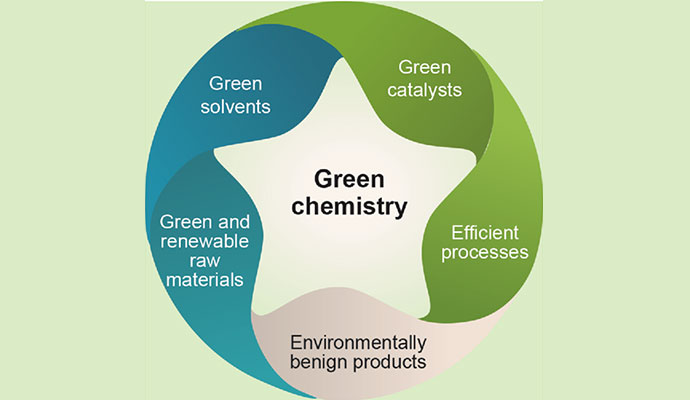
\includegraphics[width=.95\textwidth]{green-chemistry-1.jpg}
\end{figure}


\begin{itemize}
	\item \textbf{Sustainable Development} is a framework for making long-term decisions that support the health of the environment, economy, and society. It is about meeting the needs of the present without compromising the ability of future generations to meet their own needs.

	\item \textbf{Green Chemistry} aligns with sustainable development by minimizing environmental impact through the design of safer chemicals and processes. It emphasizes the reduction of waste, energy use, and the use of toxic substances in chemical production.

	\item \textbf{Economic Benefits}: Green chemistry can lead to cost savings by reducing the need for raw materials, energy, and waste disposal, while also creating opportunities for green jobs and new technologies.

	\item \textbf{Environmental Benefits}: Green chemistry helps reduce pollution at the source, thus conserving natural resources, reducing greenhouse gas emissions, and preventing environmental degradation.

	\item \textbf{Social Benefits}: By reducing exposure to hazardous chemicals, green chemistry protects public health and contributes to a higher quality of life, supporting the social aspect of sustainable development.

	\item \textbf{Life Cycle Analysis (LCA)}: Green chemistry incorporates LCA to evaluate the environmental impacts associated with all stages of a product's life, from raw material extraction to disposal, ensuring a comprehensive approach to sustainability.

	\item \textbf{Innovation and Research}: Green chemistry encourages innovation in developing new, safer chemicals and materials that are both effective and environmentally benign, fostering continuous improvement in sustainability practices.

	\item \textbf{Policy and Regulation}: Governments and regulatory bodies increasingly advocate for green chemistry principles to promote sustainable industrial practices and enforce environmental protection standards.
\end{itemize}

\section{3. Atom Economy}

\begin{figure}[H]
	\centering
	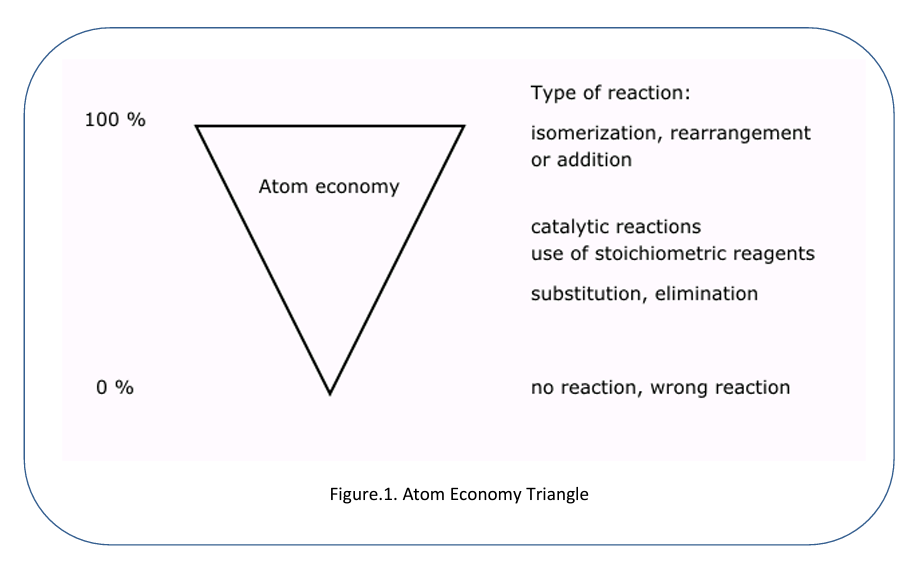
\includegraphics[width=.95\textwidth]{1670922781565.png}
\end{figure}

\textbf{Atom Economy} is a concept in green chemistry that measures the efficiency of a chemical reaction in terms of how well atoms in the reactants are incorporated into the desired final product.

\begin{itemize}
	\item \textbf{Formula}:
	      \[
		      \text{Atom Economy (\%)} = \frac{\text{Molecular weight of desired product}}{\text{Total molecular weight of all reactants}} \times 100
	      \]

	\item \textbf{Importance}: High atom economy means that fewer atoms are wasted as byproducts, leading to less waste and a more sustainable process. It is an essential metric for designing environmentally friendly chemical processes.

	\item \textbf{Example}: If a reaction converts 100\% of the reactants into the desired product without any by-products, it has 100\% atom economy. However, reactions that produce a lot of waste or by-products have lower atom economies.
\end{itemize}

\begin{itemize}
	\item \textbf{Waste Minimization}: A higher atom economy indicates less waste, making the process more sustainable and environmentally friendly. This is crucial for reducing the environmental footprint of chemical manufacturing.

	\item \textbf{Efficiency in Synthesis}: Atom economy helps in identifying more efficient synthesis routes. Reactions with higher atom economy are preferred because they require fewer raw materials and generate fewer by-products.

	\item \textbf{Cost-Effectiveness}: Reactions with high atom economy can reduce costs by minimizing the use of expensive reagents and the need for waste disposal. This economic advantage makes green chemistry more appealing to industries.

	\item \textbf{Catalysis and Atom Economy}: The use of catalysts can improve atom economy by enabling more selective reactions and reducing the number of steps required in a synthesis, which can enhance overall process efficiency.

	\item \textbf{Designing for High Atom Economy}: Chemists aim to design reactions that incorporate a higher percentage of the reactants into the desired product, thereby achieving near-total atom utilization.

	\item \textbf{Examples of High Atom Economy Reactions}: Addition reactions typically have high atom economy as they combine reactants without forming by-products. On the other hand, substitution and elimination reactions often have lower atom economy because they generate by-products.

	\item \textbf{Limitations}: Atom economy does not account for other aspects of sustainability, such as energy consumption, toxicity, or the environmental impact of solvents and reagents. Therefore, it should be used in conjunction with other metrics for a comprehensive assessment.
\end{itemize}

\section{4. Integrated Pollution Prevention and Control (IPPC)}

\textbf{Integrated Pollution Prevention and Control (IPPC)} is an approach to environmental regulation that aims to minimize pollution from various industrial sources through the use of best available techniques (BATs).


\textbf{Integrated Pollution Prevention and Control (IPPC)} is an approach to managing pollution from industrial sources to achieve a high level of environmental protection through the use of the best available techniques (BATs).

\begin{figure}[H]
	\centering
	
\includegraphics[width=.95\textwidth]{ippc_logo_green_2lines_en.jpg}
\end{figure}

\begin{itemize}
	\item \textbf{Comprehensive Regulation}: IPPC regulations require permits that address all environmental impacts (air, water, land) of industrial activities, ensuring a holistic approach to pollution control.

	\item \textbf{Best Available Techniques (BATs)}: BATs are technologies and methods that offer the most effective and advanced means of reducing emissions and waste, taking into account economic viability and technical feasibility.

	\item \textbf{Pollution Prevention at Source}: IPPC emphasizes preventing pollution at its source rather than relying on end-of-pipe solutions, leading to more sustainable industrial practices.

	\item \textbf{Resource Efficiency}: By promoting efficient use of resources, IPPC encourages industries to reduce raw material consumption, energy use, and waste generation, contributing to overall sustainability.

	\item \textbf{Continuous Improvement and Innovation}: IPPC fosters a culture of continuous improvement, where industries are encouraged to adopt new and better technologies and practices to reduce their environmental footprint over time.

	\item \textbf{Integrated Approach}: Unlike traditional regulatory approaches that focus on individual pollutants or environmental media, IPPC takes an integrated approach, considering the cumulative impact of all emissions and waste on the environment.

	\item \textbf{Permit Flexibility}: IPPC permits are flexible, allowing industries to choose how they achieve compliance, provided they meet environmental performance standards. This flexibility encourages innovation and cost-effective solutions.

	\item \textbf{Stakeholder Involvement}: IPPC involves consultation with stakeholders, including industry, regulators, and the public, to ensure that diverse perspectives are considered in decision-making, promoting transparency and accountability.

	\item \textbf{Challenges and Limitations}: Implementing IPPC can be challenging due to the need for comprehensive data, the complexity of integrated permits, and the potential for increased costs for industries. However, the long-term benefits of reduced environmental impact and enhanced sustainability often outweigh these challenges.
\end{itemize}


\section{5. Inherently Safer Design (ISD)}

\textbf{Inherently Safer Design (ISD)} is a philosophy in chemical engineering and process design that aims to eliminate or significantly reduce hazards rather than managing them with additional controls.

\begin{itemize}
	\item \textbf{Minimize}: Reduce the amount of hazardous substances in use.
	\item \textbf{Substitute}: Replace hazardous materials with less hazardous alternatives.
	\item \textbf{Moderate}: Use less hazardous conditions (e.g., lower temperatures or pressures).
	\item \textbf{Simplify}: Design processes to be less complex and therefore less prone to failure.
\end{itemize}

\textbf{Methodology}:
\begin{itemize}
	\item \textbf{Process Hazard Analysis}: Identify potential hazards and design changes to mitigate them.
	\item \textbf{Safety Reviews}: Conduct regular reviews and updates to processes as technology and regulations evolve.
	\item \textbf{Risk Assessment}: Evaluate the risks associated with different design options and choose the safest.
\end{itemize}

\section{6. Importance of Non-Conventional Energy Sources in Green Technology}

\textbf{Non-Conventional Energy Sources} such as solar, wind, geothermal, and hydroelectric power play a crucial role in promoting green technology by providing sustainable and cleaner alternatives to fossil fuels.

\begin{itemize}
	\item \textbf{Reduced Carbon Emissions}: Non-conventional energy sources produce little to no greenhouse gases compared to traditional fossil fuels, helping mitigate climate change.
	\item \textbf{Renewability}: These sources are renewable, ensuring a continuous supply of energy without depleting natural resources.
	\item \textbf{Energy Independence}: Promoting these sources reduces dependence on imported fuels, enhancing energy security.
	\item \textbf{Lower Environmental Impact}: They have a much lower impact on the environment, with fewer pollutants and reduced habitat destruction.
	\item \textbf{Supports Innovation}: The growth of renewable energy encourages innovation in green technologies, leading to more efficient and cost-effective solutions.
\end{itemize}

\begin{figure}[H]
	\centering
	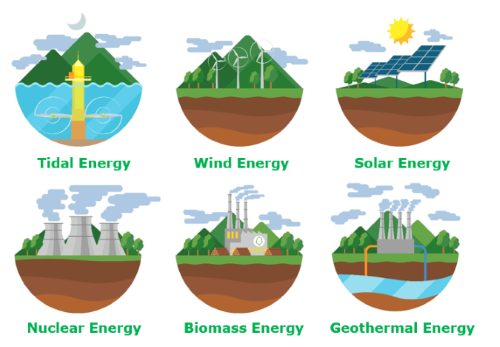
\includegraphics[width=.65\textwidth]{Sourcesofenergy5.png}
	\caption{Non conventional sources of energy}
\end{figure}

\end{document}